\section{Introduction}
This paper deals with the topic of running containerized applications on
different types of hardware with different processor architectures.  Containers
offer many advantages when it comes to running applications. They allow a high
degree of independence from the base system and still offer a lower performance
overhead than virtual machines. However, since they are also a form of
virtualization, they are not independent of the processor architecture and must
be adapted for each type of processor architecture. This is one of the problems
that limits the cross-platform use of containers.  With traditional software
operation, it was often very difficult to move software from one system to a
completely different system. The use of cloud technologies and especially
containers can make this easier to implement. Individual containers can be
moved between physical or virtual machines by container orchestration software,
and their compute power can be combined by using load balancing techniques.
The self-contained independent nature of containers also allows for migration
between cloud service providers almost seamlessly.

This is where this paper comes in. Each of the individual processor
architectures comes with its advantages and disadvantages, which can also be
tailored to specific application areas. This should be used for a smart way of
load balancing to potentially reduce the energy consumption of the running
applications. As a result, operations should be made more efficient and
operating costs should be saved.  To answer this question, this paper will
compare two processor architectures and determine their efficiency. To reduce
complexity, only one type of application will be used for the test later in the
paper. A large number of different applications with different hardware
omissions significantly increases the complexity of the experiment and also
makes it more difficult to determine the benefits of energy-efficient load
balancing.

\subsection{Significance for data centers}
A major characteristic of data centers is their
electric power consumption.
In a report from \citeauthor{shehabi2016united}, 
the data show that servers, as well as 
cooling and power provision systems each
make up 43 per cent of U.S. data center electricity use,
which together are 86 per cent. Other minor contributors
are storage drives with 11 percent and network with 3 per cent.
(see Figure \ref{fig:electricityUseDatacenter2014})
\cite{shehabi2016united}.

\begin{figure}[h]
	\centering
	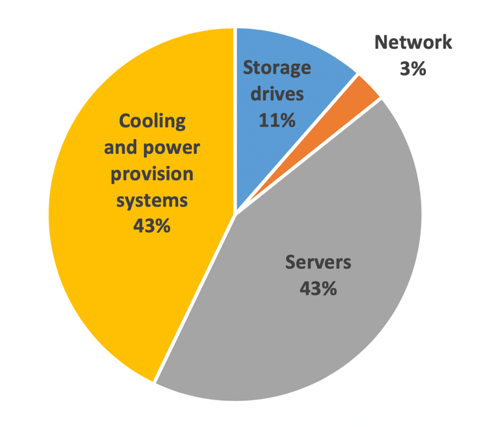
\includegraphics[width=.75\linewidth]{fig/electricityUseDatacenter2014.png}
	\caption{Fraction of U.S. data center electricity use in 2014, by end use. \cite{shehabi2016united}}
	\label{fig:electricityUseDatacenter2014}	
\end{figure}

By reducing the energy used to operate the server infrastructure, the active
operating costs for the server hardware can be lowered. However, the reduced
energy consumption also creates other benefits. Much of the energy consumed by
computers is converted into heat, which in the case of a larger data center
must be counteracted by cooling systems. With a reduction in energy consumption
and a higher performance per watt, the required cooling capacity for the
overall system also decreases. This in turn also reduces the required amount of
cooling systems and thus also space in the data center, which can be saved in
the planning or used differently. This can result in a double energy saving as
energy can be saved for both the operation and the cooling of the system at the
same time.

\subsection{Significance for private cloud and smaller companies}
By using a cluster with heterogeneous CPU architectures, older hardware could
also be used for operation. This would be particularly interesting for smaller
companies and companies that use a private cloud. Older hardware usually has a
significantly poorer performance per watt than modern hardware, but it could
still be used for operation during performance peaks and thus enable the
purchase of less new hardware.  Conversely, this could also enable operation
where some new devices are added to the old clusters, thus also reducing power
consumption.
